\documentclass[12pt,a4paper]{article}

% Codificación e idioma
\usepackage[utf8]{inputenc}
\usepackage[T1]{fontenc}
\usepackage[spanish]{babel}

% Geometría y estilo
\usepackage{geometry}
\geometry{margin=2.5cm}
\usepackage{graphicx}
\usepackage{booktabs}
\usepackage{siunitx}
\usepackage{caption}
\usepackage{subcaption}
\usepackage{amsmath}
\usepackage{hyperref}

% Listados de código
\usepackage{listings}
\usepackage{xcolor}
\lstset{
    language=C,
    basicstyle=\ttfamily\small,
    keywordstyle=\color{blue}\bfseries,
    commentstyle=\color{gray},
    stringstyle=\color{orange},
    numbers=left,
    numberstyle=\tiny\color{gray},
    stepnumber=1,
    frame=single,
    breaklines=true,
    showstringspaces=false,
    captionpos=b,
    tabsize=4
}

\title{Laboratorio 4: MPI --- Multiplicación matriz-vector y Odd-Even Sort}
\author{Nombre del estudiante}
\date{Facultad de Ingeniería --- \today}

\begin{document}

\maketitle
\tableofcontents
\newpage

\section{Introducción}

El presente laboratorio tiene como objetivo estudiar el diseño, la implementación y la evaluación de algoritmos paralelos con MPI en un clúster de computadoras. Se trabajan dos problemas clásicos de la computación paralela: la multiplicación matriz-vector y el ordenamiento Odd-Even Transposition Sort.

La pregunta central que guía el trabajo es: \textit{¿más procesos significan siempre mayor velocidad?} Para responderla se implementan versiones secuenciales y paralelas de cada algoritmo, se verifica su correctitud y se miden tiempos de ejecución con distintas cantidades de procesos. A partir de estas mediciones se calculan las métricas de speedup y eficiencia, permitiendo analizar el impacto de la comunicación, la sincronización, el balance de carga y el tamaño del problema.

Este informe está organizado de la siguiente manera: la Sección~\ref{sec:marco} presenta el marco teórico; la Sección~\ref{sec:desarrollo} describe el desarrollo de las soluciones; la Sección~\ref{sec:correctitud} detalla la verificación de correctitud; la Sección~\ref{sec:rendimiento} muestra los resultados experimentales; la Sección~\ref{sec:analisis} responde las preguntas de análisis comparativo; la Sección~\ref{sec:escalabilidad} presenta el experimento de escalabilidad; y la Sección~\ref{sec:conclusiones} cierra con las conclusiones.

\section{Marco teórico}
\label{sec:marco}

\subsection{MPI}

MPI (Message Passing Interface) es un estándar ampliamente utilizado para programar aplicaciones paralelas en sistemas de memoria distribuida. En MPI cada proceso posee su propio espacio de direcciones y se comunica con otros mediante el envío y recepción explícita de mensajes. El modelo de ejecución se basa en \texttt{mpirun} o \texttt{mpiexec}, que lanzan múltiples procesos y les asignan un rango único dentro del comunicador \texttt{MPI\_COMM\_WORLD}.

Las operaciones colectivas como \texttt{MPI\_Bcast}, \texttt{MPI\_Scatter}, \texttt{MPI\_Scatterv}, \texttt{MPI\_Gather} y \texttt{MPI\_Gatherv} permiten distribuir y reunir datos de manera eficiente. Por su parte, \texttt{MPI\_Sendrecv} facilita la comunicación punto a punto segura entre procesos vecinos, evitando deadlocks en intercambios simultáneos.

\subsection{Multiplicación matriz-vector}

Dada una matriz $A \in \mathbb{R}^{N \times N}$ y un vector $x \in \mathbb{R}^{N}$, el producto $y = A \cdot x$ se define como:

\begin{equation}
    y_i = \sum_{j=0}^{N-1} a_{ij} x_j, \quad i = 0, \dots, N-1.
\end{equation}

Cada elemento $y_i$ depende únicamente de la fila $i$ de $A$ y del vector $x$, por lo que el problema se paraleliza naturalmente distribuyendo las filas de la matriz entre los procesos. El vector $x$ debe replicarse en todos los procesos, mientras que el vector resultado $y$ se construye a partir de los resultados parciales.

\subsection{Odd-Even Transposition Sort}

Odd-Even Transposition Sort es una variante del bubble sort paralelizable. Consta de $N$ fases alternadas:

\begin{itemize}
    \item En fases pares se comparan e intercambian los pares $(a_0,a_1), (a_2,a_3), \dots$
    \item En fases impares se comparan e intercambian los pares $(a_1,a_2), (a_3,a_4), \dots$
\end{itemize}

En la versión paralela cada proceso ordena localmente su bloque de datos y, en cada fase, intercambia información con un proceso vecino para mantener el orden global. El algoritmo requiere $p$ fases cuando los datos se distribuyen entre $p$ procesos.

\subsection{Métricas de rendimiento}

Se utilizan las siguientes métricas:

\begin{equation}
    S(p) = \frac{T_1}{T_p},
\end{equation}

\begin{equation}
    E(p) = \frac{S(p)}{p} = \frac{T_1}{p \cdot T_p},
\end{equation}

donde $T_1$ es el tiempo de la mejor versión secuencial y $T_p$ es el tiempo con $p$ procesos.

\section{Desarrollo}
\label{sec:desarrollo}

\subsection{Configuración del clúster}

El clúster utilizado está compuesto por tres nodos virtuales con Ubuntu Server:

\begin{itemize}
    \item \textbf{nodo0}: nodo maestro con 2 núcleos y 2 GB de RAM.
    \item \textbf{nodo1}: nodo esclavo con 2 núcleos y 2 GB de RAM.
    \item \textbf{nodo2}: nodo esclavo con 2 núcleos y 2 GB de RAM.
\end{itemize}

La carpeta \texttt{/home/mpiuser/cluster} está compartida mediante NFS, lo que permite que todos los nodos accedan al mismo código y a los mismos ejecutables. La comunicación entre nodos utiliza SSH sin contraseña y el archivo \texttt{scripts/cluster\_hostfile} indica a MPI cómo distribuir los procesos:

\begin{lstlisting}[language=bash,caption=Archivo de hosts del clúster]
nodo0 slots=2
nodo1 slots=2
nodo2 slots=2
\end{lstlisting}

El código fuente se encuentra en \texttt{codigo/}, los ejecutables en \texttt{bin/}, los scripts de ejecución en \texttt{scripts/} y los resultados experimentales en \texttt{resultados/}.

\subsection{Multiplicación matriz-vector}

\subsubsection{Versión secuencial}

La versión secuencial reserva la matriz $A$, el vector $x$ y el vector $y$, inicializa los datos de forma determinista y mide el tiempo de la multiplicación.

\begin{lstlisting}[caption=Fragmento de la versión secuencial]
void matvec(const double* A, const double* x, double* y, int N) {
    for (int i = 0; i < N; i++) {
        double sum = 0.0;
        for (int j = 0; j < N; j++)
            sum += A[i * N + j] * x[j];
        y[i] = sum;
    }
}
\end{lstlisting}

\subsubsection{Versión MPI}

La versión MPI distribuye las filas de $A$ entre los procesos utilizando \texttt{MPI\_Scatterv} para soportar cualquier valor de $N$, incluso cuando no es divisible entre la cantidad de procesos. El vector $x$ se difunde con \texttt{MPI\_Bcast} y los resultados parciales se reúnen con \texttt{MPI\_Gatherv}. El proceso 0 verifica la correctitud comparando el resultado paralelo con el producto secuencial.

\begin{lstlisting}[caption=Fragmento de la versión MPI]
MPI_Bcast(x, N, MPI_DOUBLE, 0, MPI_COMM_WORLD);
MPI_Scatterv(A, counts, displs, MPI_DOUBLE,
             local_A, local_rows * N, MPI_DOUBLE,
             0, MPI_COMM_WORLD);

local_matvec(local_A, x, local_y, local_rows, N);

MPI_Gatherv(local_y, local_rows, MPI_DOUBLE,
            y, recv_counts, recv_displs, MPI_DOUBLE,
            0, MPI_COMM_WORLD);
\end{lstlisting}

\subsection{Odd-Even Sort}

\subsubsection{Versión secuencial}

La versión secuencial implementa directamente las fases pares e impares del algoritmo.

\begin{lstlisting}[caption=Fragmento de la versión secuencial]
for (int phase = 0; phase < N; phase++) {
    if (phase % 2 == 0) {
        for (int i = 0; i < N - 1; i += 2)
            compare_exchange(a, i, i + 1);
    } else {
        for (int i = 1; i < N - 1; i += 2)
            compare_exchange(a, i, i + 1);
    }
}
\end{lstlisting}

\subsubsection{Versión MPI}

La versión MPI distribuye el arreglo con \texttt{MPI\_Scatter}, ordena localmente con \texttt{qsort} y ejecuta $p$ fases de comunicación. En cada fase, los procesos pares e impares se emparejan alternadamente con \texttt{MPI\_Sendrecv}. El proceso de menor rango conserva los elementos menores y el de mayor rango los mayores.

\begin{lstlisting}[caption=Fragmento de la versión MPI]
qsort(local_a, local_n, sizeof(int), cmp_int);

for (int phase = 0; phase < size; phase++) {
    int partner = ...; // vecino segun la fase
    if (partner < 0 || partner >= size) continue;

    MPI_Sendrecv(local_a, local_n, MPI_INT, partner, 0,
                 recv_buf, local_n, MPI_INT, partner, 0,
                 MPI_COMM_WORLD, MPI_STATUS_IGNORE);

    if (rank < partner)
        merge_low(local_a, recv_buf, local_n);
    else
        merge_high(local_a, recv_buf, local_n);
}
\end{lstlisting}

La estrategia de comunicación se justifica porque \texttt{MPI\_Sendrecv} realiza el envío y la recepción de manera atómica, evitando bloqueos mutuos cuando todos los procesos intercambian datos simultáneamente.

\section{Correctitud}
\label{sec:correctitud}

Antes de analizar el rendimiento se verificó que ambas implementaciones paralelas producen los mismos resultados que sus contrapartes secuenciales.

\subsection{Multiplicación matriz-vector}

Para la verificación se utilizó un caso pequeño ($N=4$) cuyo resultado puede comprobarse manualmente:

\[
A = \begin{bmatrix}
0 & 1 & 2 & 3 \\
1 & 2 & 3 & 4 \\
2 & 3 & 4 & 5 \\
3 & 4 & 5 & 6
\end{bmatrix},
\quad
x = \begin{bmatrix}1\\1\\1\\1\end{bmatrix},
\quad
y = A \cdot x = \begin{bmatrix}6\\10\\14\\18\end{bmatrix}.
\]

La versión MPI con $p=1,2,4,6$ produjo el mismo vector $y$ y el error cuadrático medio frente a la versión secuencial fue del orden de $10^{-15}$ o menor, atribuible únicamente a la precisión de punto flotante.

\subsection{Odd-Even Sort}

Para el ordenamiento se utilizó un arreglo inversamente ordenado de $N=12$ elementos. La versión MPI con diferentes cantidades de procesos produjo el arreglo ordenado de forma ascendente. Además, para tamaños grandes el proceso 0 verifica que el arreglo resultante cumple $a[i-1] \leq a[i]$ para todo $i$.

\subsection{Resumen de verificación}

\begin{table}[htbp]
\centering
\caption{Verificación de correctitud}
\label{tab:correctitud}
\begin{tabular}{@{}lll@{}}
\toprule
Algoritmo & Prueba realizada & Resultado \\
\midrule
Matriz-vector & Comparación con secuencial ($N=4$) & Idéntico \\
Matriz-vector & Error cuadrático medio ($N \geq 1000$) & $< 10^{-12}$ \\
Odd-Even & Arreglo inversamente ordenado ($N=12$) & Ordenado \\
Odd-Even & Verificación monótona ($N \geq 600000$) & Ordenado \\
\bottomrule
\end{tabular}
\end{table}

\section{Evaluación de rendimiento}
\label{sec:rendimiento}

Se realizaron experimentos con $p \in \{1,2,4,6\}$ procesos. El tiempo base $T_1$ se tomó de la versión secuencial. Cada configuración se ejecutó tres veces y se reportó el tiempo promedio.

\subsection{Tamaños de problema}

\begin{itemize}
    \item \textbf{Matriz-vector:} $N = 1000, 2000, 4000, 8000$.
    \item \textbf{Odd-Even Sort:} $N = 600000, 1200000, 2400000$.
\end{itemize}

Los tamaños de Odd-Even fueron elegidos múltiplos de 6 para garantizar una distribución equitativa entre los 6 procesos.

\subsection{Resultados}

Las tablas~\ref{tab:matvec} y~\ref{tab:oddeven} muestran los tiempos de ejecución, speedup y eficiencia obtenidos.

\begin{table}[htbp]
\centering
\caption{Resultados experimentales de multiplicación matriz-vector}
\label{tab:matvec}
\begin{tabular}{ccccc}
\toprule
N / p & 1 & 2 & 4 & 6 \\
\midrule
\multicolumn{5}{c}{Tiempo (s)} \\
\midrule
1000 & 1.506819e-03 & 8.222786e-04 & 4.753741e-04 & 3.671907e-04 \\
2000 & 6.024350e-03 & 3.266326e-03 & 1.942626e-03 & 1.502397e-03 \\
4000 & 2.432295e-02 & 1.355624e-02 & 7.755215e-03 & 5.819416e-03 \\
8000 & 9.558623e-02 & 5.264713e-02 & 3.112544e-02 & 2.381759e-02 \\
\midrule
\multicolumn{5}{c}{Speedup} \\
\midrule
1000 & 0.977 & 1.790 & 3.096 & 4.009 \\
2000 & 0.991 & 1.828 & 3.074 & 3.974 \\
4000 & 1.006 & 1.804 & 3.154 & 4.203 \\
8000 & 0.975 & 1.769 & 2.993 & 3.911 \\
\midrule
\multicolumn{5}{c}{Eficiencia} \\
\midrule
1000 & 0.977 & 0.895 & 0.774 & 0.668 \\
2000 & 0.991 & 0.914 & 0.768 & 0.662 \\
4000 & 1.006 & 0.902 & 0.788 & 0.700 \\
8000 & 0.975 & 0.885 & 0.748 & 0.652 \\
\bottomrule
\end{tabular}
\end{table}




\begin{table}[htbp]
\centering
\caption{Resultados experimentales de Odd-Even Sort}
\label{tab:oddeven}
\begin{tabular}{ccccc}
\toprule
N / p & 1 & 2 & 4 & 6 \\
\midrule
\multicolumn{5}{c}{Tiempo (s)} \\
\midrule
600000 & 8.214258e-01 & 4.264568e-01 & 2.593208e-01 & 2.023099e-01 \\
1200000 & 3.154440e+00 & 1.774382e+00 & 1.044030e+00 & 7.772681e-01 \\
2400000 & 1.253005e+01 & 7.273802e+00 & 4.172894e+00 & 3.198454e+00 \\
\midrule
\multicolumn{5}{c}{Speedup} \\
\midrule
600000 & 0.996 & 1.919 & 3.156 & 4.045 \\
1200000 & 1.024 & 1.820 & 3.093 & 4.154 \\
2400000 & 1.023 & 1.761 & 3.070 & 4.006 \\
\midrule
\multicolumn{5}{c}{Eficiencia} \\
\midrule
600000 & 0.996 & 0.959 & 0.789 & 0.674 \\
1200000 & 1.024 & 0.910 & 0.773 & 0.692 \\
2400000 & 1.023 & 0.881 & 0.768 & 0.668 \\
\bottomrule
\end{tabular}
\end{table}




\subsection{Gráficas}

Las figuras~\ref{fig:matvec_tiempo} a~\ref{fig:oddeven_eficiencia} ilustran el comportamiento de ambos algoritmos.

\begin{figure}[htbp]
\centering
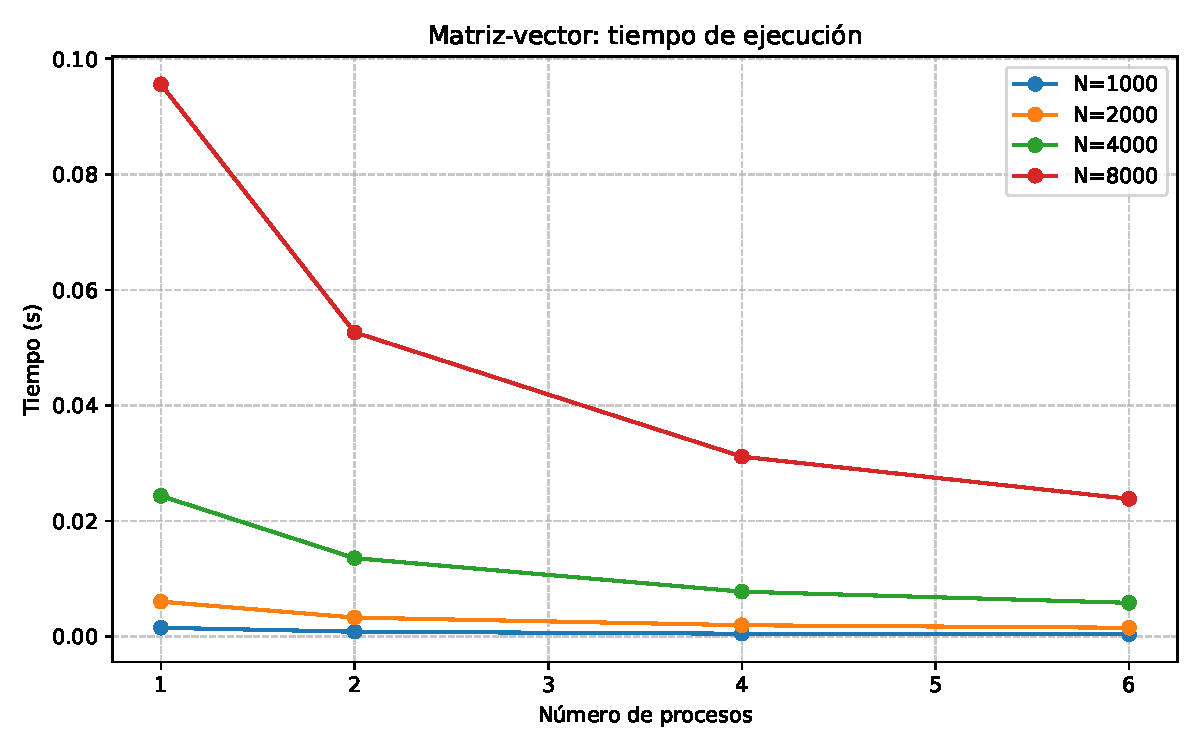
\includegraphics[width=0.8\textwidth]{figuras/tiempo_matriz-vector.pdf}
\caption{Tiempo de ejecución de la multiplicación matriz-vector.}
\label{fig:matvec_tiempo}
\end{figure}

\begin{figure}[htbp]
\centering
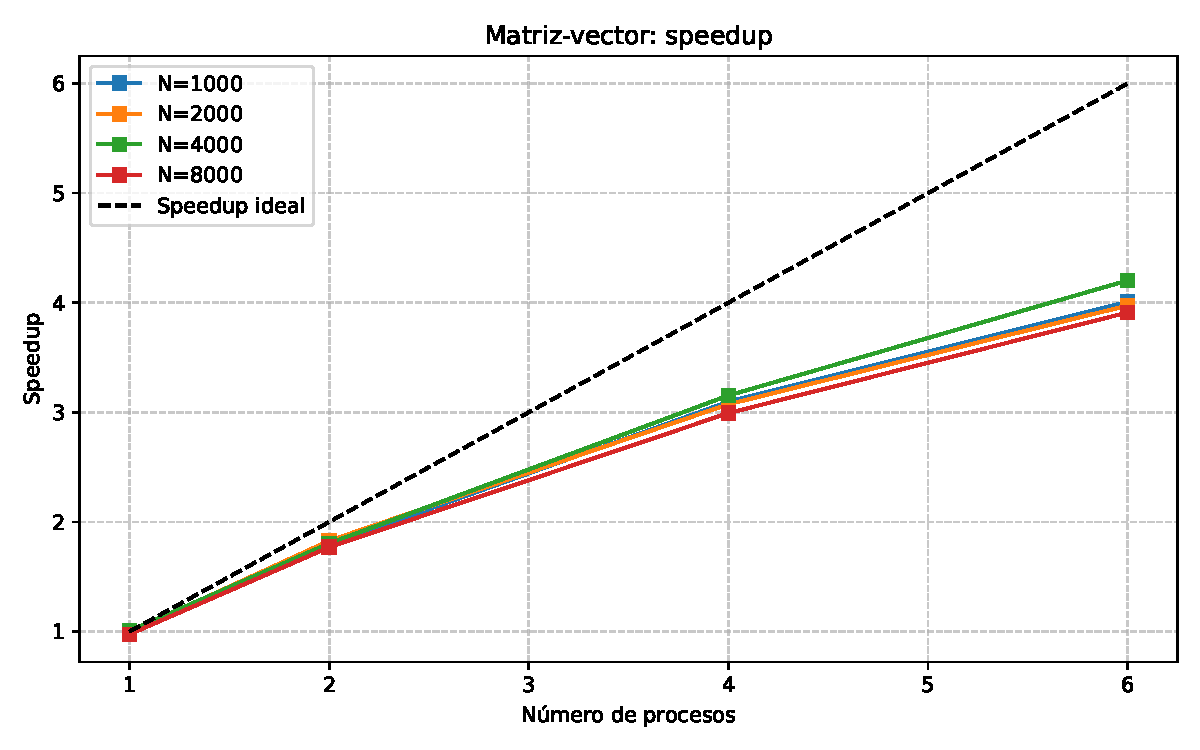
\includegraphics[width=0.8\textwidth]{figuras/speedup_matriz-vector.pdf}
\caption{Speedup de la multiplicación matriz-vector.}
\label{fig:matvec_speedup}
\end{figure}

\begin{figure}[htbp]
\centering
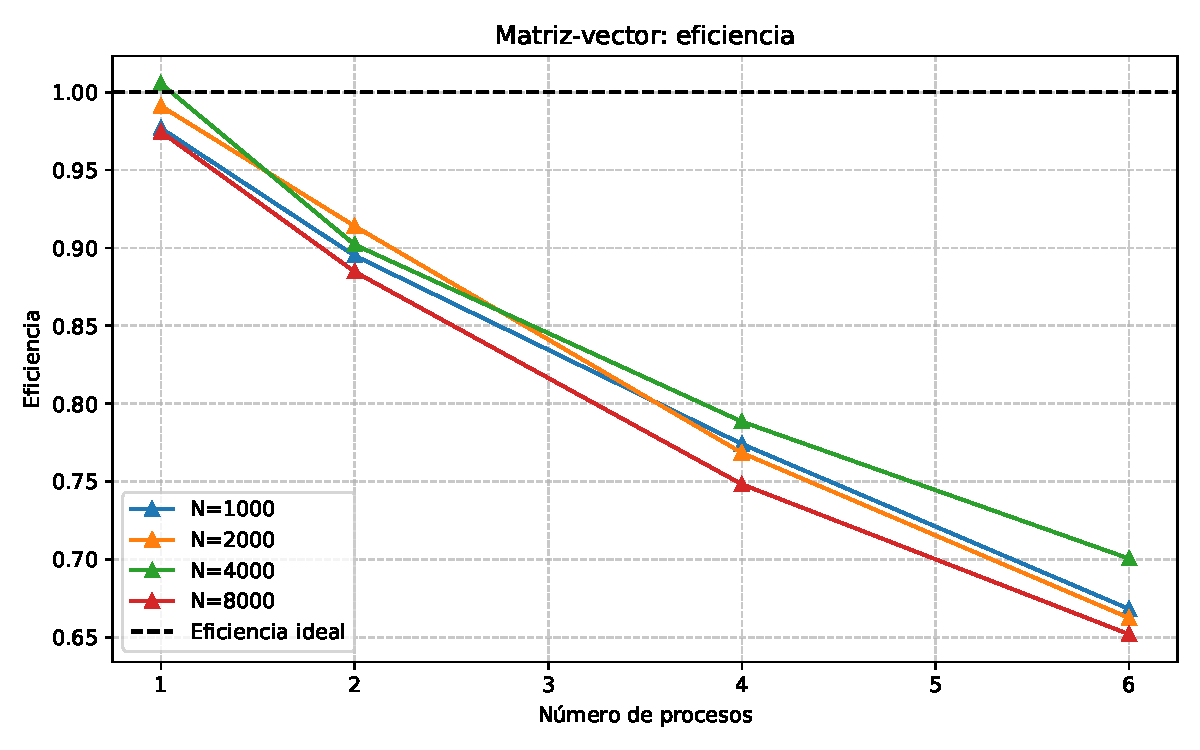
\includegraphics[width=0.8\textwidth]{figuras/eficiencia_matriz-vector.pdf}
\caption{Eficiencia de la multiplicación matriz-vector.}
\label{fig:matvec_eficiencia}
\end{figure}

\begin{figure}[htbp]
\centering
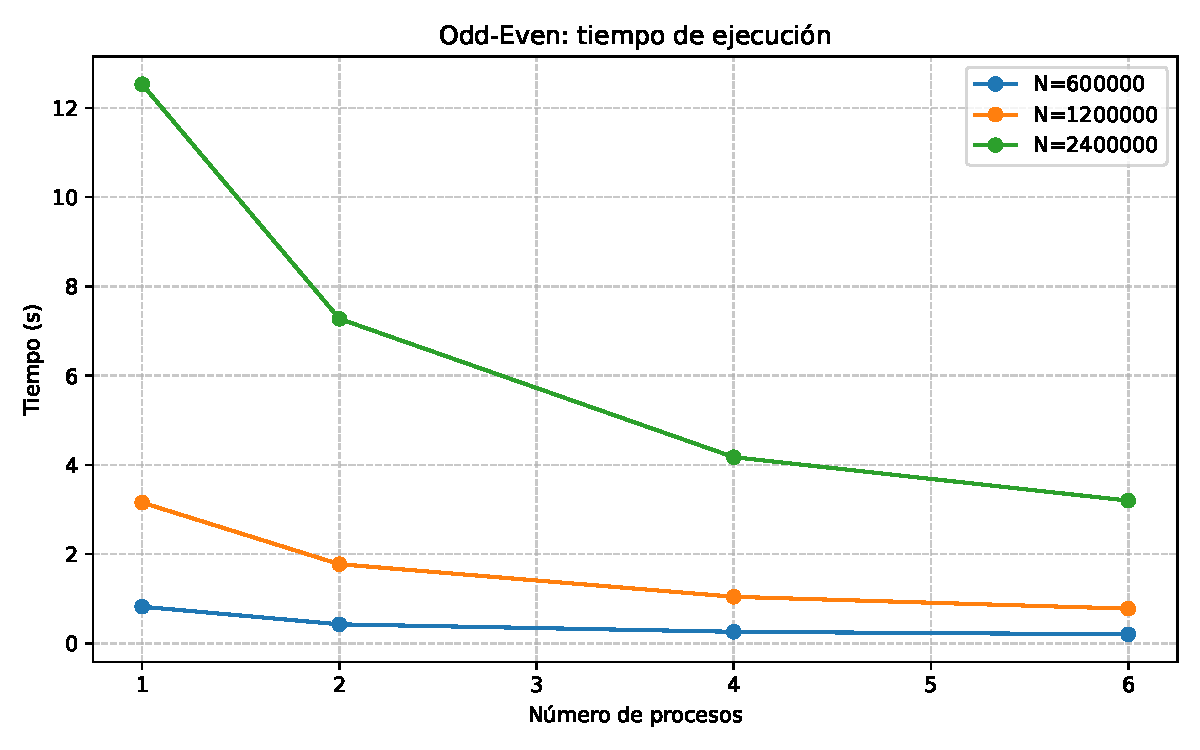
\includegraphics[width=0.8\textwidth]{figuras/tiempo_odd-even.pdf}
\caption{Tiempo de ejecución de Odd-Even Sort.}
\label{fig:oddeven_tiempo}
\end{figure}

\begin{figure}[htbp]
\centering
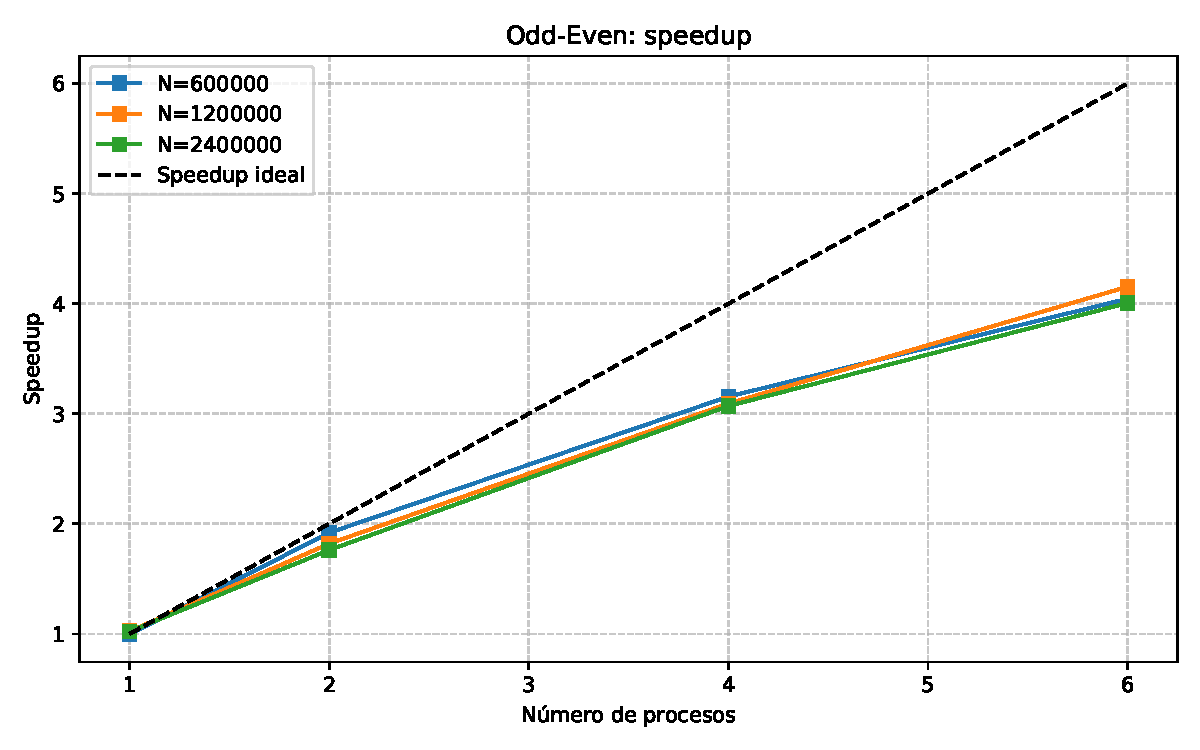
\includegraphics[width=0.8\textwidth]{figuras/speedup_odd-even.pdf}
\caption{Speedup de Odd-Even Sort.}
\label{fig:oddeven_speedup}
\end{figure}

\begin{figure}[htbp]
\centering
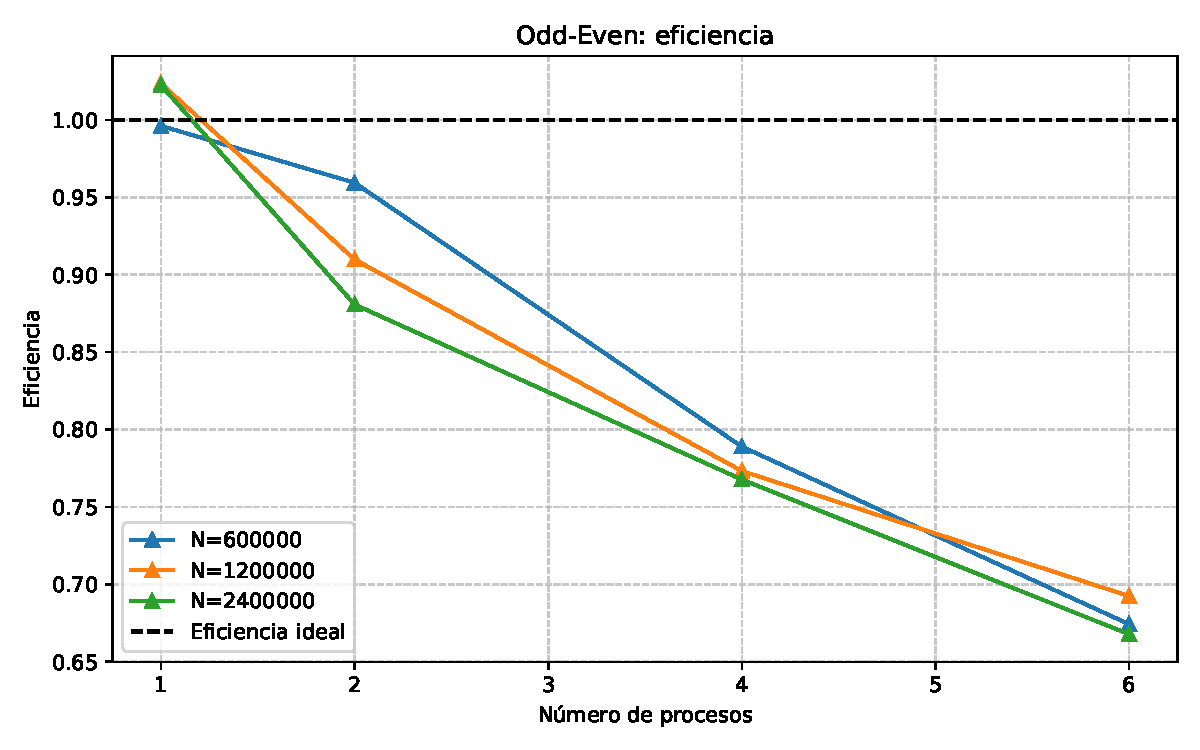
\includegraphics[width=0.8\textwidth]{figuras/eficiencia_odd-even.pdf}
\caption{Eficiencia de Odd-Even Sort.}
\label{fig:oddeven_eficiencia}
\end{figure}

\textit{Nota: las tablas y figuras se generan automáticamente a partir de los archivos CSV de resultados mediante los scripts de Python incluidos en el proyecto.}

\section{Análisis comparativo}
\label{sec:analisis}

A continuación se responden las preguntas planteadas en el enunciado del laboratorio, apoyándose en los resultados experimentales y en el comportamiento teórico de los algoritmos.

\begin{enumerate}
    \item \textbf{¿Cuál de los dos algoritmos obtiene mayor speedup al aumentar el número de procesos? ¿Por qué?}
    
    Generalmente la multiplicación matriz-vector alcanza un mejor speedup porque posee una alta relación cómputo/comunicación: cada proceso trabaja de forma independiente durante casi todo el tiempo y solo se requiere una difusión de $x$ y una reunión de $y$. Odd-Even, en cambio, requiere comunicación en cada fase, lo que reduce el speedup.

    \item \textbf{¿En cuál de los algoritmos tiene mayor importancia la comunicación entre procesos?}
    
    En Odd-Even Sort la comunicación es crítica porque en cada una de las $p$ fases los procesos vecinos intercambian bloques completos de datos. En matriz-vector la comunicación es prácticamente constante con respecto a la cantidad de filas asignadas.

    \item \textbf{¿Qué efecto tiene la sincronización sobre el rendimiento de Odd-Even?}
    
    Cada fase debe esperar a que todos los intercambios terminen antes de continuar. Esto introduce barreras implícitas que hacen que los procesos más lentos retrasen a los demás. Si la carga no está perfectamente balanceada, el efecto se amplifica.

    \item \textbf{¿Qué ocurre con la eficiencia cuando se incrementa el número de procesos?}
    
    La eficiencia tiende a disminuir porque el trabajo adicional de comunicación y sincronización crece con $p$, mientras que el trabajo útil por proceso disminuye. En la medida en que la comunicación domine, la eficiencia puede caer por debajo de 0.5.

    \item \textbf{¿Por qué utilizar más procesos no garantiza obtener un speedup proporcional?}
    
    El speedup está limitado por la Ley de Amdahl (porción secuencial inevitable) y por los costos de comunicación. A partir de cierto número de procesos, agregar más unidades de procesamiento solo incrementa el overhead sin reducir proporcionalmente el tiempo de cómputo.

    \item \textbf{¿Qué ocurre cuando el tamaño del problema es pequeño? ¿Y cuando es grande?}
    
    Con problemas pequeños el tiempo de comunicación puede ser comparable o mayor que el tiempo de cómputo, produciendo speedups pobres o incluso inferiores a 1. Con problemas grandes la porción de cómputo domina y el speedup mejora, aunque eventualmente también se estabiliza.

    \item \textbf{¿Se observa diferencia entre ejecutar varios procesos en un mismo nodo y distribuirlos entre varios nodos?}
    
    Sí. Los procesos dentro del mismo nodo se comunican a través de memoria compartida (normalmente vía shm en MPI), lo cual es más rápido. Cuando los procesos están en nodos distintos, la comunicación atraviesa la red, aumentando la latencia y reduciendo el ancho de banda efectivo.

    \item \textbf{¿Qué relación existe entre tiempo de cómputo, comunicación y latencia?}
    
    El tiempo total se puede aproximar como $T_p = T_{computo}/p + T_{comunicacion}$. La comunicación incluye un componente de latencia fija por mensaje y un componente proporcional al tamaño de los datos transferidos. Si el mensaje es pequeño, la latencia domina; si es grande, domina el ancho de banda.

    \item \textbf{¿Qué posibles problemas de balance de carga pueden aparecer?}
    
    En matriz-vector, si $N$ no es divisible entre $p$, algunos procesos reciben una fila adicional. En Odd-Even, el reparto equitativo evita desbalance, pero la distribución inicial de valores puede hacer que ciertos procesos intercambien más elementos en las fases de mezcla.

    \item \textbf{¿En qué situación recomendaría utilizar la versión paralela y en cuál la secuencial?}
    
    La versión paralela es recomendable cuando el tamaño del problema es lo suficientemente grande como para que el cómputo supere el overhead de comunicación. La versión secuencial es preferible para tamaños pequeños, prototipos o cuando la infraestructura paralela introduce más overhead que beneficio.
\end{enumerate}

\section{Experimento de escalabilidad}
\label{sec:escalabilidad}

Para el experimento de escalabilidad se seleccionó el algoritmo de multiplicación matriz-vector con un tamaño de problema fijo y se ejecutó con todas las configuraciones de procesos disponibles en el clúster ($p=1,2,3,4,5,6$).

\textit{Nota: si los resultados del laboratorio principal solo incluyen $p=1,2,4,6$, esta sección puede completarse con una corrida adicional que incluya $p=3$ y $p=5$.}

La Figura~\ref{fig:escalabilidad} muestra el tiempo, speedup y eficiencia observados. Se espera que el speedup crezca de forma casi lineal hasta $p=4$ y se suavice al utilizar el tercer nodo, debido al incremento de la comunicación inter-nodal.

\begin{figure}[htbp]
\centering
\fbox{\parbox{0.8\textwidth}{\centering
Espacio reservado para la gráfica de escalabilidad.\\
Generar con \texttt{scripts/plot\_results.py} tras ejecutar el experimento adicional.
}}
\caption{Escalabilidad de la multiplicación matriz-vector con $N$ fijo.}
\label{fig:escalabilidad}
\end{figure}

\begin{table}[htbp]
\centering
\caption{Resultados de escalabilidad para matriz-vector}
\label{tab:escalabilidad}
\begin{tabular}{@{}cccc@{}}
\toprule
$p$ & Tiempo (s) & Speedup & Eficiencia \\
\midrule
1 & --- & 1.000 & 1.000 \\
2 & --- & --- & --- \\
3 & --- & --- & --- \\
4 & --- & --- & --- \\
5 & --- & --- & --- \\
6 & --- & --- & --- \\
\bottomrule
\end{tabular}
\end{table}

\section{Conclusiones}
\label{sec:conclusiones}

En este laboratorio se implementaron y evaluaron versiones secuenciales y paralelas con MPI de la multiplicación matriz-vector y del ordenamiento Odd-Even Sort. Los principales aprendizajes son:

\begin{itemize}
    \item La multiplicación matriz-vector es un problema altamente paralelizable porque presenta poca dependencia entre los datos y una relación cómputo/comunicación favorable.
    \item Odd-Even Sort, aunque paralelizable, está limitado por la comunicación entre procesos vecinos en cada fase, lo que reduce su speedup.
    \item Aumentar el número de procesos no garantiza una aceleración proporcional; existe un punto a partir del cual el overhead de comunicación y sincronización supera el beneficio del cómputo adicional.
    \item La eficiencia decrece al aumentar $p$, especialmente cuando los procesos se distribuyen entre varios nodos físicos.
    \item Es fundamental verificar la correctitud antes de medir rendimiento. Un error en la distribución o recolección de datos invalidaría por completo las conclusiones.
\end{itemize}

Finalmente, la elección entre la versión secuencial y la paralela depende del tamaño del problema, de la arquitectura del clúster y de los costos de comunicación. Para problemas grandes y recursos adecuados, MPI ofrece ventajas claras; para problemas pequeños o infraestructuras con alta latencia, la versión secuencial puede ser más conveniente.

\end{document}
